\documentclass[french,11pt,twoside]{VcCours}

\newenvironment{ApplicationDirecte}{\textbf{Application directe du cours :}

}{}
\newcommand{\dx}{\text{d}x}
\newcommand{\dt}{\text{d}t}
\DeclareMathOperator{\e}{e}
\newcommand{\Sum}[2]{\sum_{#1}^{#2}}
\newcommand{\Int}[2]{\int_{#1}^{#2}}

\renewcommand{\trou}[1]{{\color{white}#1}}
%\renewcommand{\trou}[1]{{\color{blue}#1}}

\begin{document}

\Titre{PSI}{Promotion 2021--2022}{Mathématiques}{Chapitre 7 : Fonctions vectorielles et arcs paramétrés}

\tableofcontents
\separationTitre


Dans tout le chapitre, $I$ est un intervalle de $\mathbb{R}$ contenant au moins 
deux points et $n$ et $m$ sont deux entiers naturels non nul. Sauf indication 
contraire, $f$ désignera une application définie sur $I$ et à valeurs dans 
$\mathbb{R}^n$.

\bigskip

Le but du chapitre est :

\begin{itemize}
\item de généraliser aux fonctions à valeurs dans $\mathbb{R}^n$ la notion 
de continuité et de dérivabilité d'une fonction numérique.
\item de formaliser certaines notions géométriques utilisées dans d'autres 
matières scientifiques.
\end{itemize}

%\section{Norme sur $\mathbb{R}^n$}
%\subsection{définition de la norme euclidienne}
%Pour tout $x=(x_1, \ldots,x_n) \in \mathbb{R}^n$, on pose :
%$$ \Vert x \Vert = \sqrt{x_1^2+ x_2^2+ \cdots + x_n^2}$$
%\begin{Proposition}{} L'application $\Vert \cdot \Vert : \mathbb{R}^n \rightarrow \mathbb{R}_+$ est appelée \emph{norme euclidienne} sur $\mathbb{R}^n$. Elle vérifie les propriétés suivantes :
%\begin{itemize}
%\item Pour tout $x \in \mathbb{R}^n$, $\Vert x \Vert =0 \Rightarrow x=0_{\mathbb{R}^n}$ (\emph{séparation}).
%\item Pour tout $x \in \mathbb{R}^n$ et tout $\lambda \in \mathbb{R}$, $\Vert \lambda x \Vert = \vert \lambda \vert \Vert x \Vert$ (\emph{homogénéité}).
%\item Pour tout $(x,y) \in (\mathbb{R}^n)^2$, $\Vert x+y \Vert \leq \Vert x \Vert + \Vert y \Vert$ (\emph{inégalité triangulaire})
%\end{itemize}
%\end{Proposition}
%
%\begin{Demonstration}{} Voir le chapitre sur les espaces vectoriels normés.
%\end{Demonstration}

%\subsection{Limite d'une fonction}
%\begin{Definition}{} Soit $a \in I$ ou une extrémité de $I$. On dit que $f$ admet pour limite $\ell \in \mathbb{K}^n$ en $a$ si :
%$$ \forall \varepsilon>0, \; \exists \eta>0, \, \forall x \in I, \, \vert x-a \vert \leq \eta \Rightarrow \Vert f(x)- \ell \Vert \leq \varepsilon$$
%\end{Definition}
%
%\begin{Remarque}{} On définit aussi la notion de limite en $- \infty$ et $+ \infty$ : il suffit de comprendre que la norme euclidienne \og remplace \fg la valeur absolue dans $\mathbb{R}^n$.
%\end{Remarque}

\newpage
\section{Continuité et dérivabilité}
\subsection{Fonctions coordonnées}
Soit $\mathcal{B}=(e_1, \ldots, e_n)$ la base canonique de $\mathbb{R}^n$. Pour tout $x \in I$, il existe des réels $f_1(x), \ldots, f_n(x)$ tel que :
 $$ f(x) = (f_1(x), \ldots, f_n(x)) = \sum_{k=1}^n f_k(x) e_k$$
Les fonctions $f_k : I \rightarrow \mathbb{R}$ sont appelées les \emph{fonctions coordonnées} de $f$ dans la base canonique.
\subsection{Continuité et opérations sur les fonctions continues}
%\subsection{Continuité en un point, sur un intervalle}

\begin{Definition}{} Soit $a \in I$. On dit que $f$ est \emph{continue} en $a$ si les fonctions coordonnées de $f$ sont continues en $a$.
\end{Definition}

\begin{Remarque}{}
On définit, comme dans le cas réel, la continuité à gauche et la continuité à droite.
\end{Remarque}

%
%Soit $\mathcal{B}=(e_1, \ldots, e_n)$ la base canonique de $\mathbb{R}^n$. Pour tout $x \in I$, il existe des réels $f_1(x), \ldots, f_n(x)$ tel que :
% $$ f(x) = (f_1(x), \ldots, f_n(x)) = \sum_{k=1}^n f_k(x) e_k$$
%Les fonctions $f_k : I \rightarrow \mathbb{R}$ sont appelées les \emph{fonctions coordonnées} de $f$ dans la base canonique.

%\medskip
%
%\begin{Proposition}{continuité composante par composante} Soit $a \in I$. La fonction $f$ est continue en $a$ si et seulement si pour tout $k \in \iii{1}{n}$, $f_k$ est continue en $a$. 
%\end{Proposition}
%
%\begin{Demonstration}{} Voir chapitre sur les espaces vectoriels normés.
%\end{Demonstration}
%
%\medskip

\begin{Exemple} La fonction $f : x \mapsto (\cos(x), \sin(x))$ est continue en tout point de $\mathbb{R}$ car les fonctions cosinus et sinus le sont.
\end{Exemple}

%
%\subsection{Opérations sur les fonctions continues}

\begin{Proposition}{} Soient $a \in I$, $f : I \rightarrow \mathbb{R}^n$, $g : I \rightarrow \mathbb{R}^n$ deux fonctions continues en $a$ et $\lambda \in \mathbb{R}$. Alors $(\lambda f+g)$ est continue en $a$.
\end{Proposition}

\begin{Demonstration}{} Il suffit de se ramener aux fonctions coordonnées.
\end{Demonstration}
%
\subsection{Dérivabilité et opérations sur les fonctions dérivables}
%\subsection{Dérivabilité en un point, sur un intervalle}

\begin{Definition}{} Soit $a \in I$. On dit que $f$ est \emph{dérivable} en $a$ si ses fonctions coordonnées le sont. On définit dans ce cas le \emph{nombre dérivé} de $f$ en $a$, et on note $f'(a)$, le vecteur de $\mathbb{R}^n$ défini par :
$$ f'(a) = (f_1^{'}(a), f_2^{'}(a) ,\ldots, f_n^{'}(a))$$
\end{Definition}

%la fonction 
%$$ x \mapsto \frac{f(x)-f(a)}{x-a}$$
%définie sur $I \setminus \lbrace a \rbrace$, possède une limite en $a$. Dans ce cas, cette limite (qui est un \emph{vecteur de} $\mathbb{R}^n$), est appelé \emph{vecteur dérivée} de $f$ en $a$, et est noté :
%$$ f'(a) \quad \hbox{ ou } \quad \dfrac{\textrm{d}f}{\textrm{d}x}(a)$$
%\end{Definition}
%
%\begin{Remarque}{} Ainsi, $f$ est dérivable en $a$ et a pour vecteur dérivé $b \in \mathbb{R}^n$ si et seulement si :
%$$ \forall \varepsilon >0, \, \exists \eta > 0, \, \forall x \in I, \, \vert x- a \vert \leq \eta \Rightarrow \left\Vert \frac{f(x)-f(a)}{x-a} - b \right\Vert \leq \varepsilon$$
%\end{Remarque}

\begin{Remarque}{} On définit, comme dans le cas réel, la notion de dérivabilité à gauche et à droite. Le lien entre dérivabilité et dérivabilité à gauche/droite se généralise alors facilement.
\end{Remarque}

%\begin{Definition}{} Soient $f : I \rightarrow \mathbb{R}^n$ une fonction et $a$ un point intérieur de $I$ ou $a= \sup(I)$. On dit que que $f$ est \emph{dérivable à gauche} en $a$ si la restriction de
%$$ x \mapsto \frac{f(x)-f(a)}{x-a}$$
%à $I \cap ]- \infty,a]$ possède une limite en $a$.
%
%Dans ce cas, cette limite est un vecteur de $\mathbb{R}^n$ et on la note $f_g'(a)$.
%\end{Definition}
%
%\begin{Definition}{} Soient $f : I \rightarrow \mathbb{R}^n$ une fonction et $a$ un point intérieur de $I$ ou $a= \inf(I)$. On dit que que $f$ est \emph{dérivable à droite} en $a$ si la restriction de
%$$ x \mapsto \frac{f(x)-f(a)}{x-a}$$
%à $I \cap [a, + \infty[$ possède une limite en $a$.
%
%Dans ce cas, cette limite est un vecteur de $\mathbb{R}^n$ et on la note $f_d'(a)$.
%\end{Definition}
%
%\medskip
%
%Notons $(f_1, \ldots, f_n)$ les fonctions coordonnées de $f$ dans la base canonique :
%$$ \forall x \in I, \; f(x) = (f_1(x), \ldots, f_n(x))$$

%Soit $\mathcal{B}=(e_1, \ldots, e_n)$ la base canonique de $\mathbb{R}^n$. Pour tout $x \in I$, il existe des réels $f_1(x), \ldots, f_n(x)$ tel que :
% $$ f(x) = \sum_{k=1}^n f_k(x) e_k$$
%Les fonctions $f_k : I \rightarrow \mathbb{R}$ sont appelées les \emph{fonctions coordonnées} de $f$ dans la base canonique.
%
%\medskip

%\begin{Proposition}{dérivation composante par composante} Soit $a \in I$. La fonction $f$ est dérivable en $a$ si et seulement si pour tout $k \in \iii{1}{n}$, $f_k$ est dérivable en $a$. Dans ce cas, on a :
%$$ f'(a) = (f_1^{'}(a), f_2^{'}(a) ,\ldots, f_n^{'}(a))$$
%\end{Proposition}

\begin{Exemple} La fonction $f : x \mapsto (\cos(x), \sin(x))$ est dérivable en tout point de $\mathbb{R}$ et pour tout $x \in \mathbb{R}$, on a :
$$ f'(x) = (- \sin(x), \cos(x))$$
\end{Exemple}

\begin{Remarque}{} 
	On dit que $f$ admet pour limite $(b_1, \ldots, b_n)$ en $a$ si pour tout 
	$k \in \iii{1}{n}$, $f_k$ admet pour limite $b_k$ en $a$.
\end{Remarque}

\begin{Proposition}{développement limité et dérivabilité} Soient $a \in I$ et $b \in \mathbb{R}^n$. Les assertions suivantes sont équivalentes.

\begin{enumerate}
\item La fonction $f$ est dérivable en $a$ et $f'(a)=b$.
\item $f$ admet le développement limité suivant à l'ordre $1$ en $a$ :
$$ f(x) = f(a)+ b(x-a) + (x-a) \varepsilon(x)$$
où $\varepsilon : I \rightarrow \mathbb{R}^n$ est une fonction ayant pour limite $(0, \ldots, 0)$ en $a$.
\end{enumerate}
\end{Proposition}

\begin{Remarque}{} On note $o(x-a)$ toute fonction $x \mapsto (x-a)\varepsilon(x)$ où $\varepsilon : I \rightarrow \mathbb{R}^n$ est une fonction ayant pour limite $(0, \ldots, 0)$ en $a$.
\end{Remarque}

\begin{Corollaire}{} Si $f$ est dérivable en $a \in I$ et alors $f$ est continue en $a$. La réciproque est fausse.
\end{Corollaire}

%\subsection{Opérations sur les fonctions dérivables}

\begin{Proposition}{} Soient $a \in I$, $f : I \rightarrow \mathbb{R}^n$, $g : I \rightarrow \mathbb{R}^n$ deux fonctions dérivables en $a$ et $\lambda \in \mathbb{R}$. Alors $(\lambda f+g)$ est dérivable en $a$ et on a :
$$ (\lambda f+g)'(a) = \lambda f'(a) + g'(a) $$
\end{Proposition}

\begin{Demonstration}{} Il suffit de travailler avec les fonctions coordonnées.
\end{Demonstration}

%\begin{Proposition}{Composition par une application linéaire}
%Soient $p \in \mathbb{N}^*$ et $L : \mathbb{R}^n \rightarrow \mathbb{R}^p$ une application linéaire. Si $f : I \rightarrow \mathbb{R}^n$ est dérivable en $a \in I$ alors $L \circ f : I \rightarrow \mathbb{R}^p$ est dérivable en $a$ et on a :
%$$ (L \circ f)'(a) = L (f'(a))$$
%\end{Proposition}
%
%\begin{Demonstration}{} Voir chapitre sur les espaces normés.
%\end{Demonstration}

%\begin{Demonstration}{} Pour tout $x \in I$, $x \neq a$, on a :
%$$ \dfrac{(L \circ f)(x) - (L \circ f)(a) }{x-a} = L \left( \frac{f(x)-f(a)}{x-a} \right)$$
%par linéarité de $L$. Or $f$ est dérivable en $a$ donc :
%$$ \frac{f(x)-f(a)}{x-a} \underset{x \rightarrow a}{\longrightarrow} f'(a)$$
%Sachant que $L$ est une application linéaire sur un espace vectoriel de dimension finie, $L$ est donc continue sur $\mathbb{R}^n$ et donc en particulier en $f'(a)$. Ainsi :
%$$ L \left( \frac{f(x)-f(a)}{x-a} \right) \underset{x \rightarrow a}{\longrightarrow} L(f'(a))$$
%ce qui donne le résultat.
%\end{Demonstration}

%\begin{Remarque}{} Notons $A$ la matrice de $L$ dans les bases canoniques de $\mathbb{R}^n$ et $\mathbb{R}^p$. Si on note pour tout $t \in I$, $X(t)$ le vecteur colonne formé des coordonnées de $f(t)$ dans la base canonique. La proposition précédente s'écrit :
%$$ \forall t \in I, \; (AX)'(t) = A X'(t) $$
%\end{Remarque}
%
%\begin{Proposition}{Composition par une application bilinéaire}
%Soient $(m,p) \in (\mathbb{N}^*)^2$ et $B : \mathbb{R}^n \times \mathbb{R}^m \rightarrow \mathbb{R}^p$ une application bilinéaire. Si $f : I \rightarrow \mathbb{R}^n$ et $g : I \rightarrow \mathbb{R}^m$ sont dérivables en $a \in I$ alors $B(f,g):  I \rightarrow \mathbb{R}^p$ est dérivable en $a$ et on a :
%$$ B(f,g)'(a)= B(f'(a),g(a))+B(f(a),g'(a))$$
%\end{Proposition}
%
%\begin{Demonstration}{} Voir chapitre sur les espaces normés.
%%Pour tout $x \in I$, $x \neq a$, on a par bilinéarité de $B$ :
%%
%%\begin{align*}
%%\frac{B(f,g)(x)-B(f,g)(a)}{x-a} & =\frac{B(f(x),g(x))-B(f(a),g(x))+B(f(a),g(x))-B(f(a),g(a))}{x-a} \\
%%& = B \left( \frac{f(x)-f(a)}{x-a},g(x) \right) + B \left( f(a), \frac{g(x)-g(a)}{x-a} \right) 
%%\end{align*}
%%Les fonctions $f$ et $g$ sont dérivables (et donc continues) en $a \in I$ donc :
%%$$ g(x) \underset{x \rightarrow a}{\longrightarrow} g(a), \; \frac{f(x)-f(a)}{x-a}\underset{x \rightarrow a}{\longrightarrow} f'(a) \et \frac{g(x)-g(a)}{x-a} \underset{x \rightarrow a}{\longrightarrow} g'(a)$$
%%De plus, $B$ est bilinéaire sur $\mathbb{R}^n \times \mathbb{R}^m$ donc continue sur cet espace donc :
%%$$ \frac{B(f,g)(x)-B(f,g)(a)}{x-a}   \underset{x \rightarrow a}{\longrightarrow}  B(f'(a),g(a))+ B(f(a),g'(a))$$
%%ce qui donne le résultat.
%\end{Demonstration}
%
%\begin{Corollaire}{} Soient $f : I \rightarrow \mathbb{R}^n$ et $\alpha : I \rightarrow \mathbb{R}$ deux fonctions dérivables en $a \in I$. Alors $\alpha f $ est dérivable en $a$ et on a :
%$$ (\alpha f)'(a) = \alpha'(a) f(a) + \alpha(a) f'(a)$$
%\end{Corollaire}
%
%\begin{Demonstration}{} Bilinéarité du produit.
%\end{Demonstration}
%
%\begin{Corollaire}{} Soient $< \cdot , \cdot>$ un produit scalaire sur $\mathbb{R}^n$ et $f: I \rightarrow \mathbb{R}^n$, $g : I \rightarrow \mathbb{R}^n$ deux fonctions dérivables en $a \in I$. Alors la fonction $<f,g> \, :  I \rightarrow \mathbb{R}$ est dérivable en $a$ et :
%$$ <f,g>'(a) = <f'(a),g(a)>+<f(a),g'(a)>$$
%\end{Corollaire}
%
%\begin{Demonstration}{} $< \cdot , \cdot> \, : \mathbb{R}^n \times \mathbb{R}^n \rightarrow \mathbb{R}$ est bilinéaire.
%\end{Demonstration}
%%
%%\begin{ApplicationDirecte} Rappelons que si $< \cdot , \cdot>$ est un produit scalaire sur $\mathbb{R}^n$, on définit la norme euclidienne par :
%%$$ \forall x \in \mathbb{R}^n, \; \Vert x \Vert = \sqrt{<x,x>}$$
%%Montrer que si $f : I \rightarrow\mathbb{R}^n$ est dérivable en $a \in I$ alors $\Vert f \Vert^2$ est dérivable en $a$ et on a :
%%$$ (\Vert f \Vert^2)'(a) = 2 <f(a),f'(a)>$$
%%\end{ApplicationDirecte}
%
%\begin{nota}
%Si $x,y$ sont deux éléments de $\mathbb{R}^2$ et si $\mathcal{B}$ est une base de $\mathbb{R}^2$, on note :
%$$ \textrm{det}_{\mathcal{B}}(x,y) = \textrm{det}(\textrm{Mat}_{\mathcal{B}}(x,y))$$
%\end{nota}
%
%\begin{Corollaire}{} Soient $\mathcal{B}$ une base de  $\mathbb{R}^2$ et $f: I \rightarrow \mathbb{R}^2$, $g : I \rightarrow \mathbb{R}^2$ deux fonctions dérivables en $a \in I$. Alors la fonction $\textrm{det}_{\mathcal{B}}(f,g)$ est dérivable en $a$ et :
%$$ (\textrm{det}_{\mathcal{B}}(f,g))'(a) = \textrm{det}_{\mathcal{B}}(f'(a),g(a)) + \textrm{det}_{\mathcal{B}}(f(a),g'(a))$$
%\end{Corollaire}
%
%\begin{Demonstration}{} $\textrm{det}_{\mathcal{B}}$ est bilinéaire.
%\end{Demonstration}

\begin{Proposition}{composition} Soient $J$ un intervalle de $\mathbb{R}$, $\varphi : J \rightarrow I$ et $f : I \rightarrow \mathbb{R}^n$. Si $\varphi$ est dérivable en $x_0 \in J$ et si $f$ est dérivable en $\varphi(x_0) \in I$ alors $f \circ \varphi : J \rightarrow \mathbb{R}^n$ est dérivable en $x_0$ et on a :
$$ (f \circ \varphi)'(x_0) = \varphi'(x_0) \times (f' \circ \varphi)(x_0)$$
\end{Proposition}

\begin{Demonstration}{} Il suffit de travailler avec les fonctions coordonnées.
\end{Demonstration}

%\subsection{Fonction dérivée}

\begin{Definition}{} On dit que $f$ est \emph{dérivable} sur $I$ si $f$ est dérivable en tout point de $I$. La fonction $x \mapsto f'(x)$ est alors appelée la \emph{fonction dérivée} de $f$ et on la note $f'$.
\end{Definition}

Les résultats liées aux opérations sur les fonctions dérivables (somme, composition) se généralisent sur un intervalle.

\subsection{Dérivées d'ordre supérieur}

%\begin{Definition}{} 
%
%\begin{itemize}
%\item Sous réserve d'existence, on définit par récurrence les dérivées successives de $f$ :
%\begin{enumerate}
%\item[$\star$] $f^{(0)} =f$.
%\item [$\star$] Pour tout entier $k \geq 0$, $f^{(k+1)}=(f^{(k)})'$.
%\end{enumerate}
%\item Pour tout entier $k \geq 1$, on dit que $f$ est de \emph{classe} $\mathcal{C}^k$ sur $I$ si $f^{(k)}$ existe et est continue sur $I$.
%\item On dit que $f$ est de classe $\mathcal{C}^{\infty}$ sur $I$ si $f$ est de classe $\mathcal{C}^k$ sur $I$ pour tout entier $k \geq 1$.
%\end{itemize}
%\end{Definition}
\begin{Definition}{} Soient $k$ un entier naturel et $a \in I$. On dit que $f$ est de \emph{classe} $\mathcal{C}^k$ en $a$ si toutes ses fonctions coordonnées le sont. On pose alors :
$$  f^{(k)}(a) = (f_1^{(k)}(a), f_2^{(k)}(a) ,\ldots, f_n^{(k)}(a))$$
Si la fonction $f$ est de classe $\mathcal{C}^k$ en tout point de $I$, on dit que $f$ est de classe $\mathcal{C}^k$ sur $I$ et cela définit une fonction $f^{(k)} : I \rightarrow \mathbb{R}$.
\end{Definition}

\begin{Definition}{} Une fonction $f : I \rightarrow \mathbb{R}^n$ est de classe $\mathcal{C}^{\infty}$ sur $I$ si elle est de classe $\mathcal{C}^k$ pour tout entier $k \geq 0$.
\end{Definition}
%
%\begin{Proposition}{classe $\mathcal{C}^k$ composante par composante} 
%\begin{itemize}
%\item La fonction $f$ est de classe $\mathcal{C}^k$ sur $I$ si et seulement si pour tout $j \in \iii{1}{n}$, $f_j$ est de classe $\mathcal{C}^k$ sur $I$. Dans ce cas, pour tout $i \in \iii{1}{k}$ et tout $a \in I$,
%$$ f^{(i)}(a) = (f_1^{(i)}(a), f_2^{(i)}(a) ,\ldots, f_n^{(i)}(a))$$
%\item La fonction $f$ est de classe $\mathcal{C}^{\infty}$ sur $I$ si et seulement si pour tout $j \in \iii{1}{n}$, $f_j$ est de classe $\mathcal{C}^{\infty}$ sur $I$. Dans ce cas, pour tout $i \in \mathbb{N}^*$  et tout $a \in I$,
%$$ f^{(i)}(a) = (f_1^{(i)}(a), f_2^{(i)}(a) ,\ldots, f_n^{(i)}(a))$$
%\end{itemize}
%\end{Proposition}



\begin{Proposition}{} 
\begin{itemize}
\item Soient $f : I \rightarrow \mathbb{R}$, $g : I \rightarrow \mathbb{R}$ deux fonctions de classes $\mathcal{C}^k$ sur $I$ et $\lambda \in \mathbb{R}$. Alors $(\lambda f+g)$ est de classe $\mathcal{C}^k$ sur $I$ et on a pour tout $i \in  \iii{1}{k}$ et tout $a \in I$,
$$ (\lambda f+g)^{(i)}(a) = \lambda f^{(i)}(a) + g^{(i)}(a) $$
\item  Soient $f : I \rightarrow \mathbb{R}$, $g : I \rightarrow \mathbb{R}$ deux fonctions de classes $\mathcal{C}^{\infty}$ sur $I$ et $\lambda \in \mathbb{R}$. Alors $(\lambda f+g)$ est de classe $\mathcal{C}^{\infty}$ sur $I$ et on a pour tout $i \in \mathbb{N}^*$ et tout $a \in I$,
$$ (\lambda f+g)^{(i)}(a) = \lambda f^{(i)}(a) + g^{(i)}(a) $$
\end{itemize}
\end{Proposition}

\begin{Remarque}{} Les ensembles $\mathcal{C}^k(I, \mathbb{R}^n)$ (resp. $\mathcal{C}^{\infty}(I, \mathbb{R}^n)$) des fonctions de classes $\mathcal{C}^k$ (resp. $\mathcal{C}^{\infty}$) de $I$ dans $\mathbb{R}^n$ sont des sous-espaces vectoriels de $\mathcal{F}(I, \mathbb{R}^n)$.
\end{Remarque}

%\begin{Proposition}{Composition par une application linéaire}
%Soient $p \in \mathbb{N}^*$ et $L : \mathbb{R}^n \rightarrow \mathbb{R}^p$ une application linéaire. 
%\begin{itemize}
%\item Si $f : I \rightarrow \mathbb{R}^n$ est de classe $\mathcal{C}^k$ sur $I$ alors $L \circ f : I \rightarrow \mathbb{R}^p$ est de classe $\mathcal{C}^k$ sur $I$ et on a pour tout $i \in \iii{1}{k}$ et tout $a \in I$,
%$$ (L \circ f)^{(i)}(a) = L (f^{(i)}(a))$$
%\item  Si $f : I \rightarrow \mathbb{R}^n$ est de classe $\mathcal{C}^{\infty}$ sur $I$ alors $L \circ f : I \rightarrow \mathbb{R}^p$ est de classe $\mathcal{C}^{\infty}$ sur $I$ et on a pour tout $i \in \mathbb{N}^*$ et tout $a \in I$,
%$$ (L \circ f)^{(i)}(a) = L (f^{(i)}(a))$$
%\end{itemize}
%\end{Proposition}
%
%\begin{Theoreme}{formule de Leibniz}
%Soient $(m,p) \in (\mathbb{N}^*)^2$ et $B : \mathbb{R}^n \times \mathbb{R}^m \rightarrow \mathbb{R}^p$ une application bilinéaire.  Si $f : I \rightarrow \mathbb{R}^n$ et $g : I \rightarrow \mathbb{R}^m$ sont de classes $\mathcal{C}^k$ sur $I$ alors $B(f,g):  I \rightarrow \mathbb{R}^p$ est de classe $\mathcal{C}^k$ sur $I$ et on a :
%$$ B(f,g)^{(k)}(a)=  \sum_{i=0}^{k} \binom{k}{i} B(f^{(i)},g^{(k-i)})$$
%\end{Theoreme}

%\begin{ApplicationDirecte} Démontrer le résultat précédent par récurrence sur $k \geq 1$.
%\end{ApplicationDirecte}

\begin{Proposition}{composition} Soient $J$ un intervalle de $\mathbb{R}$, $\varphi : J \rightarrow I$ et $f : I \rightarrow \mathbb{R}^n$. Si $\varphi$ est de classe $\mathcal{C}^k$ (resp. $\mathcal{C}^{\infty}$) sur $J$ et si $f$ est de classe $\mathcal{C}^k$ (resp. $\mathcal{C}^{\infty}$) sur I alors $f \circ \varphi : J \rightarrow \mathbb{R}^n$ est de classe $\mathcal{C}^k$ (resp. $\mathcal{C}^{\infty}$) sur $J$. 
\end{Proposition}

\newpage
\section{Norme sur \texorpdfstring{$\mathbb{R}^n$}{Rⁿ}}
Pour tout $x=(x_1, \ldots,x_n) \in \mathbb{R}^n$, on pose :
$$ \Vert x \Vert = \sqrt{x_1^2+ x_2^2+ \cdots + x_n^2}$$
\begin{Proposition}{} L'application $\Vert \cdot \Vert : \mathbb{R}^n \rightarrow \mathbb{R}_+$ est appelée \emph{norme euclidienne} sur $\mathbb{R}^n$. Elle vérifie les propriétés suivantes :
\begin{itemize}
\item Pour tout $x \in \mathbb{R}^n$, $\Vert x \Vert =0 \Rightarrow x=0_{\mathbb{R}^n}$ (\emph{séparation}).
\item Pour tout $x \in \mathbb{R}^n$ et tout $\lambda \in \mathbb{R}$, $\Vert \lambda x \Vert = \vert \lambda \vert \Vert x \Vert$ (\emph{homogénéité}).
\item Pour tout $(x,y) \in (\mathbb{R}^n)^2$, $\Vert x+y \Vert \leq \Vert x \Vert + \Vert y \Vert$ (\emph{inégalité triangulaire})
\end{itemize}
\end{Proposition}

\begin{Demonstration}{} Voir le chapitre sur les espaces vectoriels normés.
\end{Demonstration}

\medskip 

Pour $n=2$, on retrouve la norme usuelle :
$$ \Vert (x,y) \Vert = \sqrt{x^2+y^2}$$

\section{Arcs paramétrés}

\subsection{Généralités}

\begin{Definition}{} Soit $k \in \mathbb{N}^*$ ou $k = + \infty$.

\begin{itemize}
\item On appelle \emph{arc paramétré} de classe $\mathcal{C}^k$ tout couple $\Gamma=(I,f)$ où $I$ est un intervalle de $\mathbb{R}$ et $f : I \rightarrow \mathbb{R}^n$ une fonction de classe $\mathcal{C}^k$ sur $I$.
\item On appelle \emph{support} de l'arc paramétré l'image de $f$ par $I$, c'est-à-dire l'ensemble généralement noté $\Gamma$ défini par :
$$ \Gamma = f(I) = \lbrace f(t) \, \vert \,  t \in I\rbrace$$
\end{itemize}
\end{Definition}

\begin{Remarque}{} Le support est parfois appelé courbe paramétrée et $f$ est alors appelé un paramétrage de celle-ci. Sans soulever des détails théoriques, $f(t)$ peut être vu comme un point de $\mathbb{R}^n$ dans certains cas et comme un vecteur dans d'autre cas.
\end{Remarque}

\medskip

\begin{Exemple} Soient $A=(x_A,y_A) \in \mathbb{R}^2$ et $v= (\alpha, \beta) \in \mathbb{R}^2$ non nul. Posons :
	\[\application{f}{\R}{\R^2}{t}{(x_A,y_A) + t (\alpha, \beta)}\]
Alors $(\mathbb{R},f)$ est une courbe paramétrée de classe $\mathcal{C}^{\infty}$ sur $\mathbb{R}$ et son support est la droite du plan $\mathbb{R}^2$ passant par $A$ et de vecteur directeur $v$.
\end{Exemple}

\medskip

\begin{Exemple} Posons :
	\[\application{f}{[0,2\pi]}{\R^2}{t}{(\cos(t), \sin(t))}\]
Déterminons le support de $([0,2\pi],f)$.

\vspace{4cm}
\end{Exemple}

\begin{Remarques}{}
\begin{itemize}
\item Le vecteur $f(t)$ désigne un point du support : on dit que c'est le \emph{point de paramètre} $t$. Attention : un point peut avoir plusieurs paramètres.
\item Attention à ne pas confondre l'arc paramétré et son support : on peut paramétrer de plusieurs manières le même support mais le paramétrage donne une information sur la manière dont on parcourt ce support, donne la \og dynamique \fg .
\item Si le paramètre $t$ parcourant l'intervalle $I$ est le temps, $\Gamma$ représente alors le mouvement d'un point dans $\mathbb{R}^n$. Le support donne alors la \emph{trajectoire} de ce mouvement.
\end{itemize}
\end{Remarques}{}

\begin{Definition}{} Soient $k \in \mathbb{N}^* \cup \lbrace + \infty \rbrace$ et $(I,f)$ un arc paramétré de classe $\mathcal{C}^k$ de support $\Gamma$.

\begin{itemize}
\item Un point $f(t)$ de $\Gamma$ est dit \emph{régulier} si $f'(t) \neq (0,0, \ldots, 0)$. Sinon, il est dit \emph{stationnaire} (ou \emph{singulier}).
\item Si tous les points de $\Gamma$ sont réguliers, on dit que $\Gamma$ est \emph{régulier}.
\end{itemize}
\end{Definition}

\begin{Remarque}[\alerte]{}
	Si $f(t_1) = f(t_2)$ (on dit qu'on est en présence d'un \emph{point double}) avec $t_1 \neq t_2$ alors le point $f(t_1)$ peut être régulier sans que $f(t_2)$ le soit.
\end{Remarque}

\medskip

Dans la suite, $\Vert \cdot \Vert$ sera la norme euclidienne sur $\mathbb{R}^n$.

\medskip

\begin{TheoremeDefinition}{tangente en un point régulier}
Soient $a \in I$ et $f(a)$ un point régulier de $\Gamma$. Alors :
$$ \dfrac{f(t)-f(a)}{\Vert f(t)-f(a) \Vert} \underset{t \rightarrow a^+}{\longrightarrow} \frac{f'(a)}{\Vert f'(a) \Vert} \et  \dfrac{f(t)-f(a)}{\Vert f(t)-f(a) \Vert} \underset{t \rightarrow a^-}{\longrightarrow} \frac{-f'(a)}{\Vert f'(a) \Vert}$$
La droite passant par $f(a)$ et dirigée par le vecteur $f'(a)$ (ou pas tout autre vecteur non nul colinéaire à $f'(a)$) est appelée \emph{tangente} à $\Gamma$ en $f(a)$.
\end{TheoremeDefinition}

\begin{Demonstration}{} Pour $t$ proche de $a$, sachant que $f$ est dérivable en $a$, on a :
$$ f(t)=f(a)+f'(a)(t-a)+o(t-a)$$
avec $f'(a) \neq 0_{\mathbb{R}^n}$. Ainsi :
$$ f(t)-f(a)= (t-a) (f'(a)+o(1))$$
Pour $t>a$ assez proche de $a$, $f'(a)+o(1) \neq  0_{\mathbb{R}^n}$ (car tend vers $f'(a) \neq  0_{\mathbb{R}^n}$) et donc $f(t)-f(a) \neq  0_{\mathbb{R}^n}$ et on a par homogénéité de la norme :
$$  \dfrac{f(t)-f(a)}{\Vert f(t)-f(a) \Vert} = \frac{t-a}{t-a} \times \frac{f'(a)+o(1)}{\Vert f'(a)+o(1)\Vert} = \frac{f'(a)+o(1)}{\Vert f'(a)+o(1)\Vert} \underset{t \rightarrow  a^+}{\longrightarrow} \frac{f'(a)}{\Vert f'(a) \Vert}$$
ce qui donne le résultat (on fait de même pour $a^{-}$).
\end{Demonstration}

\medskip

\begin{Remarque}{}
D'un point de vue cinématique, $f'(a)$ est le vecteur vitesse (instantanée) du point mobile au temps $a$. Ainsi, si la vitesse du point mobile est non nulle, la trajectoire  admet une tangente en $f(t)$ dirigée par $f'(a)$. Si l'arc paramétré est de classe $\mathcal{C}^2$ sur $I$, $f''(a)$ est le vecteur accélération du point mobile $M$ au temps $a$.
\end{Remarque}

\medskip

\begin{Exemple} Posons :
\[\application{f}{[0,2\pi]}{\R^2}{t}{(\cos(t), \sin(t))}\]
Dans un exemple précédent, on a montré que le le support $([0,2\pi],f)$ était le cercle de centre l'origine et de rayon $1$. L'arc paramétré est de classe $\mathcal{C}^{\infty}$ sur $[0,2\pi]$. On a pour tout $t \in [0, 2 \pi]$,
$$ f'(t) = (-\sin(t),\cos(t))$$
Le point $f(t)$ est régulier car $f'(t) \neq (0,0)$. Remarquons aussi :
$$ <f(t),f'(t)> = 0$$
On obtient le tracé suivant :

\begin{center}
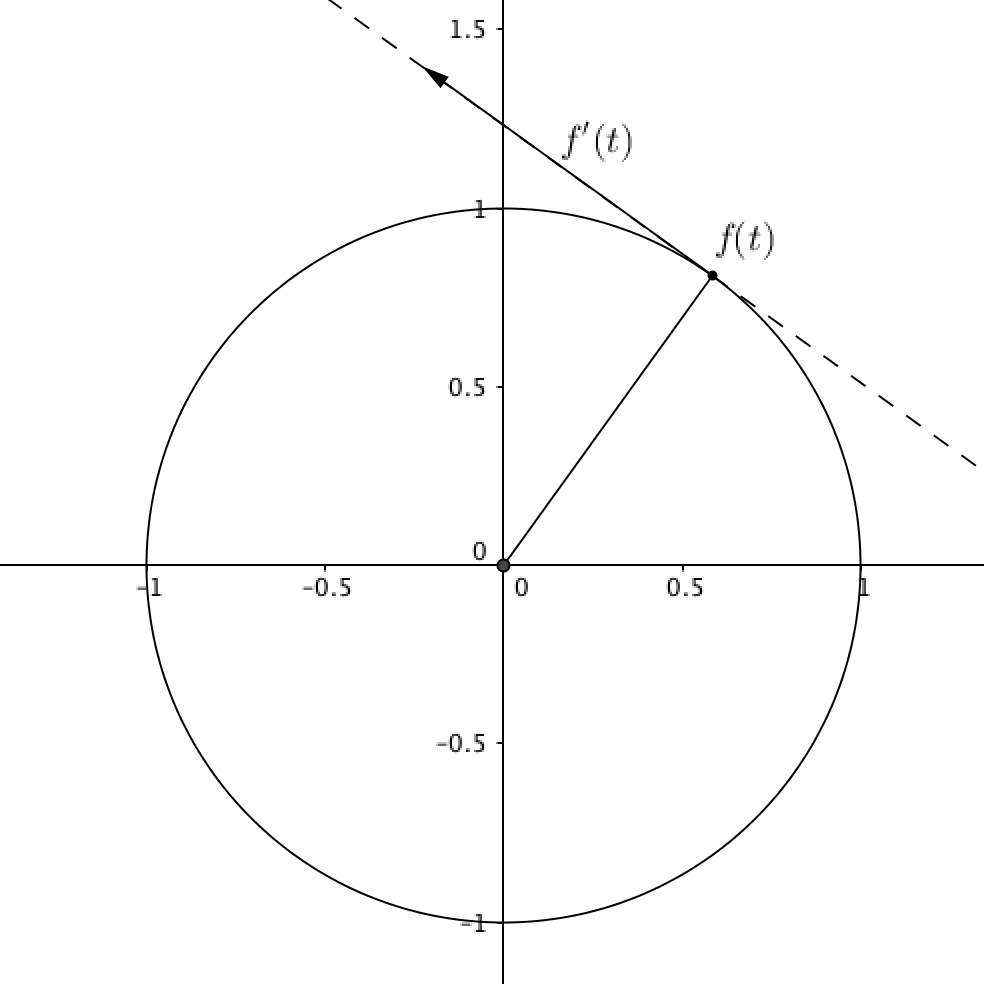
\includegraphics[scale=0.4]{cercle}
\end{center}
\end{Exemple}

%\begin{Remarque}{} Dans l'exemple précédente, on a pour tout $t \in [0,2\pi]$,
%$$\Vert f(t) \Vert^2=1$$
%Sachant que $f$ est dérivable sur $[0,2\pi]$, on retrouve que :
%$$ 2<f(t),f'(t)>=0$$
%\end{Remarque}

\subsection{Étude locale d'un arc paramétré du plan}
Dans toute la suite, on considère une fonction $f : I \rightarrow \mathbb{R}^2$ de classe $\mathcal{C}^k$ et on pose $f=(x,y)$ ($x$ et $y$ sont les fonctions coordonnées de $f$ dans la base canonique). D'après la formule de Taylor (appliquée à $x$ et $y$ et donc obtenu pour $f$), on a pour tout $a \in I$,
$$ f(t)  \underset{a}{=} \sum_{j=0}^k \dfrac{f^{(j)}(a)}{j!} (t-a)^j+ (t-a)^k \varepsilon(t)$$
où $\varepsilon : I \rightarrow \mathbb{R}^2$ a pour limite $(0,0)$ en $a$.

\medskip

On suppose maintenant l'existence de deux entiers $1 \leq p <q \leq k$ tels que :
\begin{itemize}
\item Pour tout $j \in \iii{1}{p-1}$, $f^{(j)}(a)=(0,0)$.
\item Pour tout $j \in \iii{p+1}{q-1}$, $f^{(p)}(a)$ et $f^{(j)}(a)$ sont liées.
\item La famille $(f^{(p)}(a), f^{(q)}(a))$ est libre.
\end{itemize}

\medskip

Si $(p,q)$ existe, ce couple est unique et on dit que $p$ et $q$ sont les \emph{entiers caractéristiques} de $\Gamma$. 

\medskip

On a dans ce cas :

\begin{itemize}
\item $f^{(p)}(a) \neq (0,0)$.
\item Il existe $\alpha_{p+1}, \ldots, \alpha_{q-1}$ tels que :
$$ f^{(p+1)}(a) = \alpha_{p+1} f^{(p)}(a), \ldots,  f^{(q-1)}(a)= \alpha_{q-1} f^{(p)}(a)$$
\end{itemize}
On obtient par un développement limité de $f$ en $a$ à l'ordre $q$ (par troncature) : 
$$ f(t) =  f(a) + \dfrac{(t-a)^p}{p!} f^{(p)}(a) \left( 1 + \sum_{j=p+1}^{q-1} \alpha_j \dfrac{(t-a)^{j-p}}{j!} \right) + \dfrac{(t-a)^q}{q!} f^{(q)}(a) + (t-a)^q \eta(t)$$
où $\eta : I \rightarrow \mathbb{R}^2$ a pour limite $(0,0)$ en $a$.

\begin{Remarque}{} 
La droite passant par $M(a)$ et dirigée par $f^{(p)}(a)$ est ici aussi appelée 
\emph{tangente} à $\Gamma$ en $f(a)$ (cela généralise ce que l'on définit 
pour $p=1$ quand le point est régulier). On montre avec l'égalité précédente que :
$$ \dfrac{f(t)-f(a)}{\Vert f(t)-f(a) \Vert} \underset{t \rightarrow a^+}{\longrightarrow} 
\frac{f^{(p)}(a)}{\Vert f^{(p)}(a) \Vert} \et  \dfrac{f(t)-f(a)}{\Vert f(t)-f(a) \Vert} 
\underset{t \rightarrow a^-}{\longrightarrow} \frac{(-1)^p f^{(p)}(a)}{\Vert f^{(p)}(a) \Vert}$$
\end{Remarque}

En travaillant dans le repère $(f(a), f^{(p)}(a), f^{(q)}(a))$, on déduit de l'égalité précédente que pour tout $t \in I$, $t$ proche de $a$, le point $f(t)$ a pour coordonnées :
$$ \begin{pmatrix}
\dfrac{(t-a)^p}{p!}+o((t-a)^p) \\
\dfrac{(t-a)^q}{q!}+o((t-a)^q) \\
\end{pmatrix} = \begin{pmatrix}
(t-a)^p \left( \dfrac{1}{p!} + o(1) \right) \\
(t-a)^q \left( \dfrac{1}{q!} + o(1) \right) \\
\end{pmatrix}$$
Cette égalité signifie que pour tout $t \in I$, $t$ proche de $a$ et différent de $a$, le signe de la première coordonnée est du signe de $(t-a)^p$ et la seconde est du signe de $(t-a)^q$. Ainsi, déterminer $p$ et $q$, permet de décrire l'allure de la courbe au voisinage de $f(a)$ selon la parité de $p$ et $q$.

\newpage
\begin{center}
\textbf{Allure de la courbe au voisinage d'un point}
\end{center}
\begin{multicols}{2}

\begin{center}
$f(a)$ est un \emph{point ordinaire}

($p$ impair et $q$ pair)
\end{center}

\begin{center}
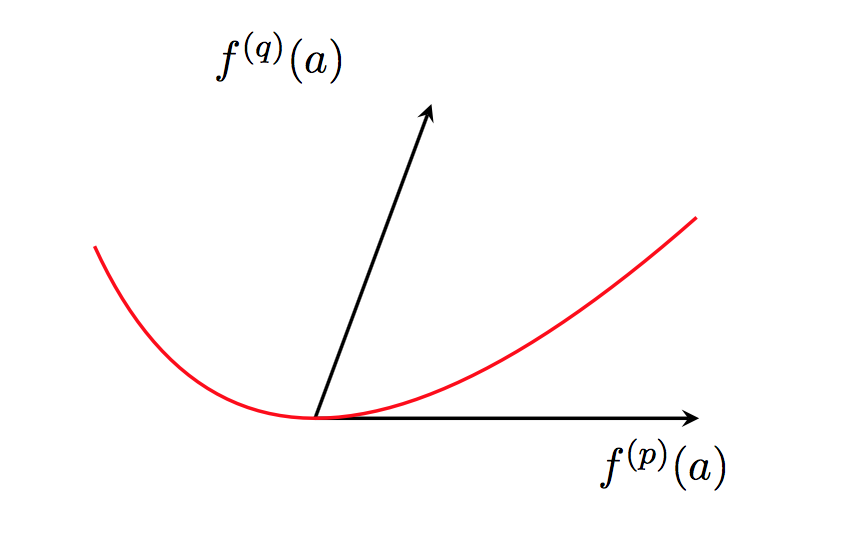
\includegraphics[scale=0.45]{im1}
\end{center}

\columnbreak

\begin{center}
$f(a)$ est un \emph{point de rebroussement de première espèce}

($p$ pair et $q$ impair)
\end{center}

\begin{center}
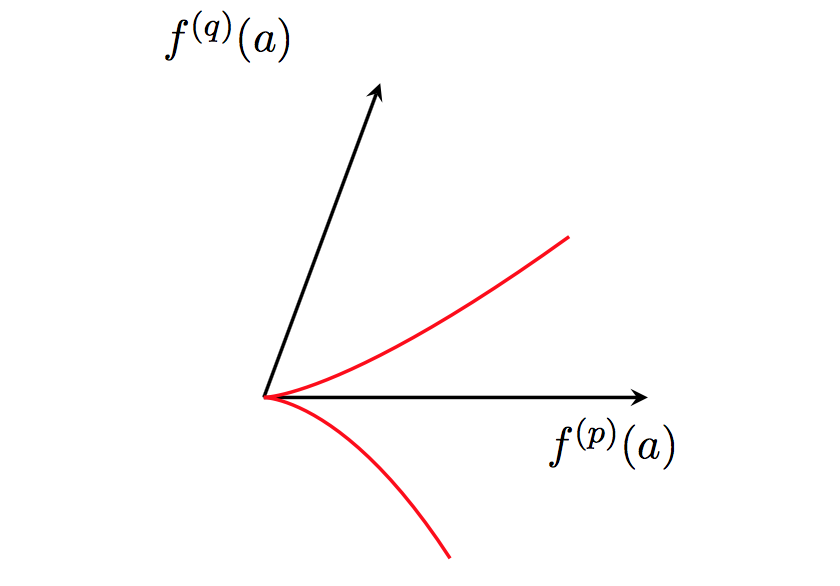
\includegraphics[scale=0.45]{im3}
\end{center}
\end{multicols}



\begin{multicols}{2}


\begin{center}
$f(a)$ est un \emph{point d'inflexion}

($p$ impair et $q$ impair)

\end{center}

\begin{center}
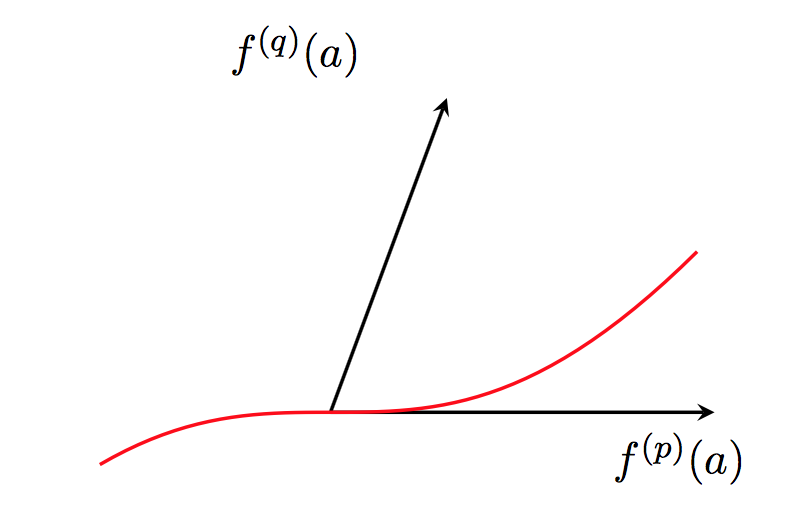
\includegraphics[scale=0.45]{im2}
\end{center}

\columnbreak

\begin{center}
$f(a)$ est un \emph{point de rebroussement de deuxième espèce} 

($p$ pair et $q$ pair)
\end{center}

\begin{center}
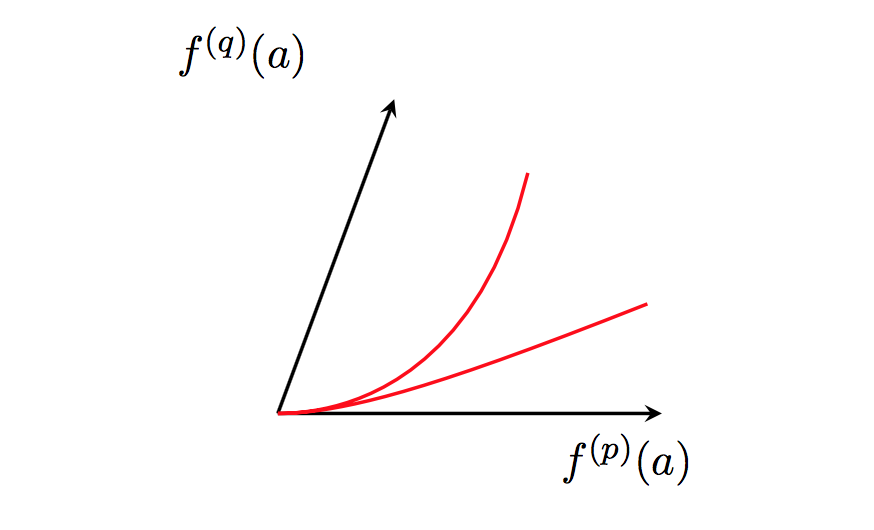
\includegraphics[scale=0.45]{im4}
\end{center}
\end{multicols}

\medskip

\begin{Exemple} Considérons l'arc paramétré suivant :
\[\application{f}{\R}{\R^2}{t}{(t^2+ \cos(t), t- \sin(t))}\]
Déterminons les points singuliers de celui-ci et donnons l'allure de la courbe au voisinage de chacun de ces points.

%\vspace*{9cm}
\end{Exemple}

\newpage
\subsection{Branches infinies}
On note toujours $f=(x,y)$.

\begin{Definition}{} On dit que $\Gamma$ possède une \emph{branche infinie} en $a$ si :
$$ \lim_{t \rightarrow a} \Vert f(t) \Vert = + \infty$$
\end{Definition}

\begin{Remarque}{} On peut distinguer $a^{-}$ et $a^{+}$.
\end{Remarque}

\medskip

\begin{Methode}{Étude d'une branche infinie}
 \begin{enumerate}
 \item Si $x$ ou $y$ a une limite finie en $a$ :
 \begin{itemize}
 \item On dit que $\Gamma$ possède une \emph{asymptote verticale} d'équation $x=m \in \mathbb{R}$ en $a$ si :
 $$ \lim_{t \rightarrow a} x(t)=m \; \hbox{ et } \; \lim_{t \rightarrow a} y(t) =\pm  \infty $$
  \item On dit que $\Gamma$ possède une \emph{asymptote horizontale} d'équation $y=m \in \mathbb{R}$ en $a$ si :
 $$ \lim_{t \rightarrow a} x(t)=\pm \infty \; \hbox{ et } \; \lim_{t \rightarrow a} y(t) = m$$
 \end{itemize}
 \item Si $x$ et $y$ ont des limites infinies :
 \begin{itemize}
 \item On dit que $\Gamma$ possède une \emph{branche parabolique} de direction $(Ox)$ en $a$ si :
 $$ \lim_{t \rightarrow a} \dfrac{y(t)}{x(t)} = 0$$
 \item  On dit que $\Gamma$ possède une \emph{branche parabolique} de direction $(Oy)$ en $a$ si :
 $$ \lim_{t \rightarrow a} \dfrac{y(t)}{x(t)} = \pm \infty$$
 \item Si $\lim_{t \rightarrow a} \dfrac{y(t)}{x(t)} = m \in \mathbb{R}^*$ :
 \begin{enumerate}
 \item Si $\lim_{t \rightarrow a} y(t)-mx(t) = p \in \mathbb{R}$, on dit que $\Gamma$ possède une \emph{asymptote} d'équation $y=mx+p$ en $a$.
  \item Si $\lim_{t \rightarrow a} y(t)-mx(t) = \pm \infty$, on dit que $\Gamma$ possède une \emph{direction asymptotique} d'équation $y=mx+p$ en $a$.
 \end{enumerate}
 \end{itemize}
 \end{enumerate}
\end{Methode}

\begin{Exemple} Étudions les branches infinies $\pm \infty$ de l'arc paramétré $f=(x,y)$ où pour tout $t \in \mathbb{R}$,
$$ x(t) = -4t^2+4t \; \hbox{ et } \; y(t)=-t^3+t$$

\newpage
\vspace*{5cm}
\end{Exemple}


%\begin{Exemple} Étudions les branches infinies en $\pm \infty$ de la courbe paramétrée définie par $f=(x,y)$ ou pour tout $t \in \mathbb{R}$,
%$$ x(t) = -4t^2+4t \; \hbox{ et } \; y(t)=-t^3+t$$
%
%\vspace{5cm}
%\end{Exemple}


\begin{Exemple} Étudions les branches infinies en $\dfrac{\pi}{2}$ de l'arc paramétré définie par $f=(x,y)$ où pour tout $t \in ]0, \pi/2[$,
$$ x(t) = \tan(t)+\sin(t) \; \hbox{ et } \; y(t)=\dfrac{1}{\cos(t)}$$

%\vspace*{12cm}
\end{Exemple}
\newpage

\subsection{Construction d'un arc paramétré du plan}
\begin{Methode}{Étude d'un arc paramétré du plan}
	
On se donne un arc paramétré du plan $\Gamma =(I,f)$ où $f=(x,y)$.

\begin{enumerate}
\item On détermine l'ensemble de définition de $f$.
\item On détermine l'ensemble d'étude de $f$ (en utilisant la périodicité ou d'éventuelles symétries) :
\begin{itemize}
\item Si $x$ et $y$ sont $T$-périodiques, on restreint l'étude à un intervalle de longueur de $T$, par exemple $[-T/2,T/2]$.
\item Si $I$ est symétrique par rapport à $0$, on peut restreindre l'étude à $I \cap \mathbb{R}_+$ dans les cas suivants :
\begin{enumerate}
\item Si $x$ et $y$ sont paires : l'étude sur $I \cap \mathbb{R}_+$ permet de tracer toute la courbe.
\item Si $x$ et $y$ sont impaires : la courbe est symétrique par rapport à l'origine.
\item Si $x$ est paire et $y$ impaire : la courbe est symétrique par rapport à l'axe des abscisses.
\item Si $x$ est impaire et $y$ paire : la courbe est symétrique par rapport à l'axe des ordonnées.
\item Si pour tout $t \in I$, $x(-t)=y(t)$ et $y(-t)=x(t)$ alors la courbe est symétrique par rapport à la droite d'équation $y=x$.
\end{enumerate}
\end{itemize}
\item On étudie $f$ : variations et limites aux bornes de $x$ et $y$. On en déduit les tangentes verticales et horizontales à la courbe.
\item On détermine les points réguliers et singuliers et l'allure de la courbe au voisinage des points singuliers.
\item On étudie les branches infinies. Si $y=mx+p$ est asymptote, le signe de $y(t)-mx(t)-p$ donne la position de la courbe par rapport à la droite d'équation $y=mx+p$.
\item On peut chercher les (éventuels) points doubles :
$$ x(t_1)=x(t_2) \et y(t_1)=y(t_2) \; \hbox{ où } t_1 \neq t_2$$
C'est généralement pénible.
\item On effectue le tracé.
\end{enumerate}
\end{Methode}

\subsection{Un exemple de tracé}
Étudions l'arc paramétré du plan de composantes :
$$ x : t \mapsto \dfrac{1}{1-t^2}, \; \, y : t \mapsto \dfrac{t^3}{1-t^2}$$

\textbf{Ensemble de définition :}

\vspace{1cm}

\newpage
\textbf{Ensemble d'étude :}

\vspace{2cm}

\textbf{Étude de $x$ et $y$ :}

\vspace{12cm}


\textbf{Allure de la courbe autour du ou des points singuliers : }

\vspace{6cm}

\newpage
\textbf{Étude des branches infinies :}

\vspace{7cm}


\textbf{Tracé de la courbe :}

\vspace{6cm}



\subsection{Longueur d'un arc}
Dans ce paragraphe, $(I,f)$ est un arc paramétré avec $f : I \rightarrow \mathbb{R}^n$ et on considère $\mathbb{R}^n$ muni de sa norme euclidienne.

\begin{Definition}{} Supposons que $(I,f)$ soit de classe $\mathcal{C}^1$. 

\begin{enumerate}
\item Si $I=[a,b]$, on appelle \emph{longueur} de $\Gamma$ le réel $\int_{a}^b \Vert f'(t) \Vert \dt$.
\item Si $I$ est un intervalle quelconque, on appelle \emph{longueur} de $\Gamma$ le réel $\int_{I} \Vert f'(t) \Vert \dt$ lorsque l'intégrale associée est convergente (voir chapitre associé).
\end{enumerate}
\end{Definition}

\begin{Remarque}{} $t \mapsto \Vert f'(t) \Vert$ est continue car $f$ est de classe $\mathcal{C}^1$ sur $I$.
\end{Remarque}

\newpage
\begin{Exemple} Considérons : 
	\[\application{f}{[0,2\pi]}{\R^2}{t}{(\cos(t), \sin(t))}\]
Déterminons la longueur de l'arc associé :

\vspace*{4cm}
\end{Exemple}
\end{document}
